\section{Shared face coefficients}\label{cs:shared}
A fixed finite collection of boxes may be assigned genuine labels
\(s_e\), with every occurrence of each face variable identified.
Keep designated zero faces exactly zero. Let \(t_f\) be the ordinary
coefficient targets, and choose a single positive radius \(\rho_f\)
for each remaining face. Require that the sum of the two outer moduli
is positive in every box; a zero pattern killing both outer variables
is outside Theorem~\ref{lc:main}. Cauchy's coefficient formula gives
\[
 \left|[L^t]\prod_eH_{V,s_e}(L;\sigma_e)\right|
 \le\prod_f\rho_f^{-t_f}
       \sup_{|L_f|=\rho_f}\prod_e|H_{V,s_e}(L;\sigma_e)|.
\]
Theorem~\ref{lc:main} applies at this shared radius vector. If
\(t_f/N\to\tau_f\), the uniform real-cube upper rate is at most
\[
                      \sum_eA_{s_e}(\rho)-\sum_f\tau_f\log\rho_f .
\]
The number of boxes is fixed before \(N\) grows, so their errors sum
to \(o(N)\). For finitely many sector strings, take the maximum of
these sums before bounding their finite sum. This keeps correlations
between genuine labels; no Cartesian enlargement is needed.

This argument gives an upper bound for each prescribed sector choice.
The coefficientwise comparison \eqref{lc:central-coefficientwise} applies
to the central sector. The one-sided estimates remain bounds on values;
we have not proved coefficientwise domination for them.

\subsection{The marked triangulation and its central coefficient}
Let $\mathcal T$ be a finite simple oriented triangulation of the sphere.
A perfect matching of its dual pairs its triangles across $R$ edges.
Its $R+2$ vertices are called faces, following their role in the original
diagram. Choose a nonmatching edge $uv$ as the mark. The two face
variables $L_u,L_v$ are set to zero; the remaining $R$ variables are
ordinary. The order at a matched pair is $(x,b,c,y)$: its triangles
are $(x,b,y)$ and $(x,c,y)$, with their induced opposite orientations
along the matching edge $xy$. Repeated occurrences of a face always
denote the same variable.
In particular $x+y>0$ on the positive ordinary radii of every pair:
otherwise its matching edge would be the unique edge $uv$, which is
the nonmatching mark. Each pair also has a nonmonomial triangle.
If one outer face is protected, only one other zero remains, so at
least one middle is positive; if both outers are positive, both
triangles are nonmonomial.

Use the operator and face polynomial of Section~\ref{lc:source}, with
$d=N-1$ and $J=\lfloor d/2\rfloor$. The central sector is equivalently
the set of paths with $i\le J$ and $d-j\le J$. At each matched edge
we select this sector of the same divided difference $V_N$.

Put $\sigma_e=-2\cos(2\pi\delta_e)$ and define the raw central coefficient
\begin{equation}\label{sa:coefficient}
 C_N(\delta)=
 \left[\prod_{f\ne u,v}L_f^d\right]
 \left.\prod_{e=1}^R H_{V,\mathrm C}
       (L_{x_e},L_{b_e},L_{c_e},L_{y_e};\sigma_e)
                  \right|_{L_u=L_v=0}.
\end{equation}
This definition includes its sign $(-1)^{dR}$. Its identification as a
contribution to the original marked evaluation, with cups, caps and
framing still present, is the exact diagram theorem
\cite[Theorem 9.1 and Corollary 9.2]{FinitePaper}. The coefficient itself is
the object of the present analytic theorem.

\begin{figure}[t]
\centering
% Native TikZ source. Incidence drawing, not a circle packing.
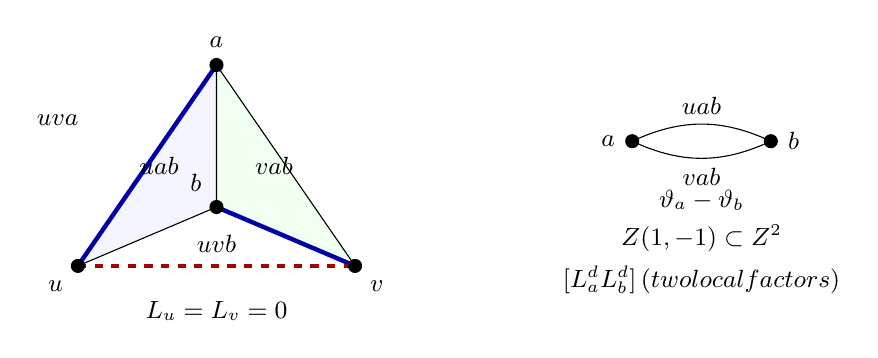
\begin{tikzpicture}[scale=.88, every node/.style={font=\small},
  vertex/.style={circle,fill=black,inner sep=1.8pt},
  matching/.style={draw=blue!65!black,line width=1.6pt},
  marked/.style={draw=red!65!black,dashed,line width=1.2pt}]
  \coordinate (u) at (-2,0);
  \coordinate (v) at (2,0);
  \coordinate (a) at (0,2.9);
  \coordinate (b) at (0,.85);
  \fill[blue!4] (u)--(a)--(b)--cycle;
  \fill[green!6] (v)--(a)--(b)--cycle;
  \draw[matching] (u)--(a);
  \draw[matching] (v)--(b);
  \draw[marked] (u)--(v);
  \draw (u)--(b)--(a)--(v);
  \node[vertex,label=below left:$u$] at (u) {};
  \node[vertex,label=below right:$v$] at (v) {};
  \node[vertex,label=above:$a$] at (a) {};
  \node[vertex,label=above left:$b$] at (b) {};
  \node at (-.83,1.45) {$uab$};
  \node at (.83,1.45) {$vab$};
  \node at (0,.32) {$uvb$};
  \node[anchor=east] at (-1.85,2.1) {$uva$};
  \node at (0,-.65) {$L_u=L_v=0$};
  \begin{scope}[xshift=7cm]
    \coordinate (aa) at (-1,1.8);
    \coordinate (bb) at (1,1.8);
    \draw (aa) to[bend left=25] node[above] {$uab$} (bb);
    \draw (aa) to[bend right=25] node[below] {$vab$} (bb);
    \node[vertex,label=left:$a$] at (aa) {};
    \node[vertex,label=right:$b$] at (bb) {};
    \node[align=center] at (0,.65)
      {$\vartheta_a-\vartheta_b$\\[3pt]$\mathbb Z(1,-1)\subset\mathbb Z^2$};
    \node at (0,-.2) {$[L_a^dL_b^d]\,(\text{two local factors})$};
  \end{scope}
\end{tikzpicture}

\caption{A combinatorial tetrahedral sphere and its ordinary phase graph.
The vertices $u,v,a,b$ name shared face variables. The marked edge $uv$
(red, dashed) sets $L_u=L_v=0$; the two blue matching edges are $ua$
and $vb$. The outer face of the planar drawing is the triangle $uva$.
The two triangles with two ordinary vertices, $uab$ and $vab$, compare the same
ordinary phases $\vartheta_a,\vartheta_b$, giving two copies of the
primitive difference row $(1,-1)$. Their coefficients add in the
Hessian, while the quotient angular measure remains
$d\vartheta_b/(2\pi)$ after $\vartheta_a=0$. The coefficient target is
$L_a^dL_b^d$, with each variable shared by the two local factors.
The edge lengths in this combinatorial drawing do not prescribe the radii
in the variational problem.}
\label{sa:shared-figure}
\end{figure}

Here is the sole positive-radius input. It can be supplied by the
complete packing of the marked triangulation, but is stated analytically
so that the theorem can be used without a geometric normalization.
Use the triangle function $\mathcal Q$ defined in \eqref{lc:entropy},
with every protected face kept exactly zero.
Choose positive ordinary radii $\rho_f$ such that
\begin{equation}\label{sa:stationarity}
 \mathcal F(L)=\sum_{e=1}^R
     \{\calQ(x_e,b_e,y_e)+\calQ(x_e,c_e,y_e)\}
                         -\sum_{f\ne u,v}\log L_f
 \quad\text{is stationary at }L=\rho
\end{equation}
modulo common scale. Set $\Phi=\mathcal F(\rho)$.
Zeros remain exactly zero. The diagram and radii are fixed before $N$
tends to infinity.

\begin{theorem}[Asymptotic of the shared central coefficient]\label{sa:main}
Under these hypotheses there is a fixed complex polydisk about zero
and, for all sufficiently large $N$, holomorphic functions $A_N$ and
holomorphic $(R-1)$-by-$(R-1)$ matrices $H_N$ on it such that
\begin{equation}\label{sa:H1}
 C_N(\delta)=
 \frac{(-1)^{dR}N^{2R}e^{NA_N(\delta)}}
 {(2\pi N)^{(R-1)/2}\sqrt{\det H_N(\delta)}}
                         (1+O(N^{-1})).
\end{equation}
The relative error is holomorphic and uniform on smaller closed
polydisks. The square root continues the positive face Hessian at zero.
The actions are separately even and real on the real chart, and
$A_N\to A_0$, $H_N\to H_0$ locally uniformly with every fixed derivative.
The face Hessian $H_0(0)$ is positive definite. Moreover
\begin{equation}\label{sa:hessian}
 \begin{aligned}
 A_0(0)&=\Phi,\qquad A_0''(0)=-2\operatorname{diag}(\kappa_e),\\
 \kappa_e&=\frac{\pi\bigl(\sqrt{b_e(x_e+y_e)+x_ey_e}
                    +\sqrt{c_e(x_e+y_e)+x_ey_e}\bigr)}
                    {x_e+y_e}>0.
 \end{aligned}
\end{equation}
All face values in the last expression are at $\rho$.

For every $0<\eta<1/2$ there are $\gamma_\eta,\tau_\eta>0$ such that,
for all sufficiently large integer levels,
\begin{equation}\label{sa:H2}
 |C_N(x+\ii y)|\le e^{N(\Phi-\gamma_\eta)}
 \quad(x\in[-1/2,1/2]^R,\ \max_e|x_e|\ge\eta,
                       \ \max_e|y_e|\le\tau_\eta).
\end{equation}
Fixed derivatives have the corresponding bounds on smaller domains.
There is no prime-level restriction and no change of normalization
between even and odd levels.
\end{theorem}

We define the finite actions directly from the actual local polynomial.
They are not asserted to equal a separately constructed approximate
fold interpolation. In particular no value-only interpolation is
differentiated to obtain a normal.

